\section{Implementation} 

\subsection{Step 1 : Application Workflow and UI Design}
	
The application was conceptualized and prototyped using Justinmind Prototyper. 

Initially we did the UI design of the application in JustinMind tool. 
When we launch the Android application, Screen shown in Figure 1 will be shown in the app which we call the Main screen. The rationale behind the UI design of this first screen is to show the user all the top recipes to get their attention. 
Now the user can click the Navigation drawer panel at the top left corner of the screen.
Following which all the recipe categories such as Cheap Eats,Healthy recipes, Quick and Easy recipes and Cuisines will be shown on the left fragment view of the screen. 
The rationale behind providing these recipe categories are users often tend to find search functionality to search for appropriate recipes by keyword search based mechanism. 
By having the popular dishes and more frequently used recipe categories, we are offering users easy way of accessing and finding their recipes and showing an element of surprise.
The reason behind choosing the Healthy recipes as recipe category is that users who are on a diet plan can easily find the list of healthy recipes with our application instead of searching for a recipe and later figuring out if that recipe is healthy or not.The reason behind choosing the Cheap Eats recipe is for cooks who are trying to save money and on a budget plan, we will show the recipes that are cheap. 
Similarly, we have provided Quick and Easy recipe category for the cooks who are running out of time and in a hurry to make some dish. 

Once the cook selects one of the recipe categories, any one of the screens in the figures 3,4,5,6 will be shown in the app. 
Now, the cook can select any one of the recipes listed on the screen. As they do that, the recipe review screen, as shown in Figure 7 will be launched. The recipe review screen displays the image of the recipe, list of ingredient and their quantities required to prepare the dish. Now, the cook can review the ingredients and check if they have it or need to buy them from groceries. When the cook decides to prepare the dish, he will collect all the ingredients listed in the recipe review screen and press 'Cook' button.

Now, the user sees the recipe cards screen as shown in Figure 8. This screen lists out all the steps of the cooking process. Each recipe card shows a step in the cooking process. Each recipe card consists of cooking directions, time needed for that step and the image describing the step. 

So, the users can scroll down the screen seeing one card at a time on the screen. When they click the start button at the top, timer keeps ticking down until it reaches to zero. On reaching zero, the app automatically scrolls down to the recipe card of the next step.This enables the user to concentrate fully on his cooking.

We also added functionality to 'Pause' the timer in cases when the user has to leave the kitchen. When the user clicks the 'Pause' button, the timer is paused. The user clicks the 'Resume' button again as shown in Figure 9. So, using this application, user can have smooth cooking experience.

\begin{figure}[ht!]
	\centering
	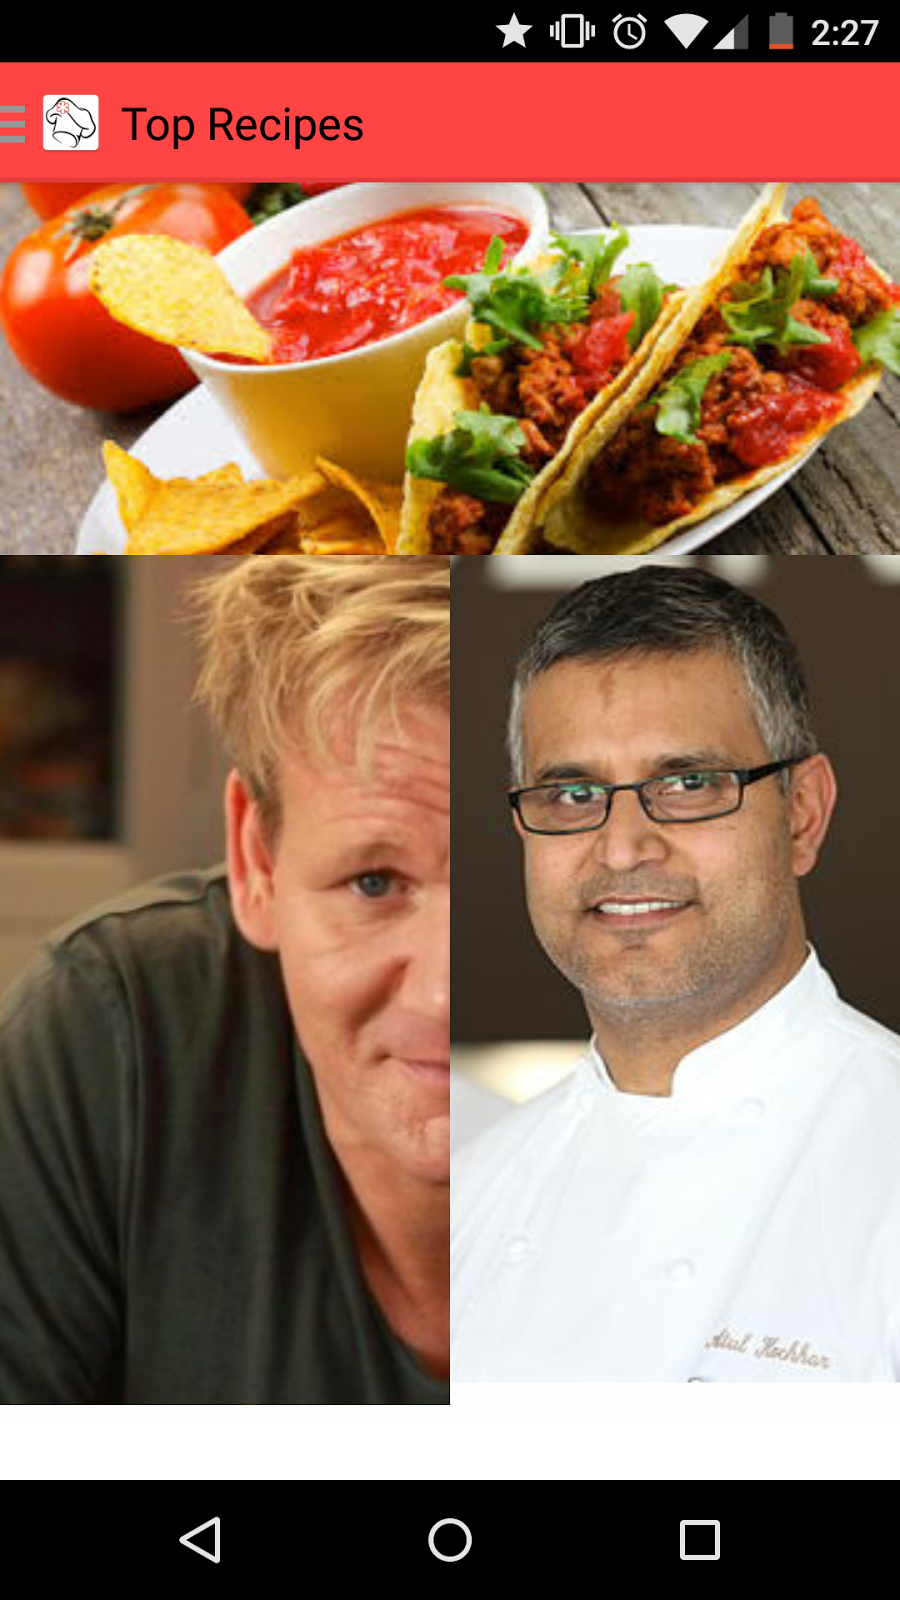
\includegraphics[width=0.3\textwidth, height=0.3\textheight]{images/main_screen.png}
	\caption{Main Screen \label{overflow}}
\end{figure}
	
\begin{figure}[ht!]
	\centering
	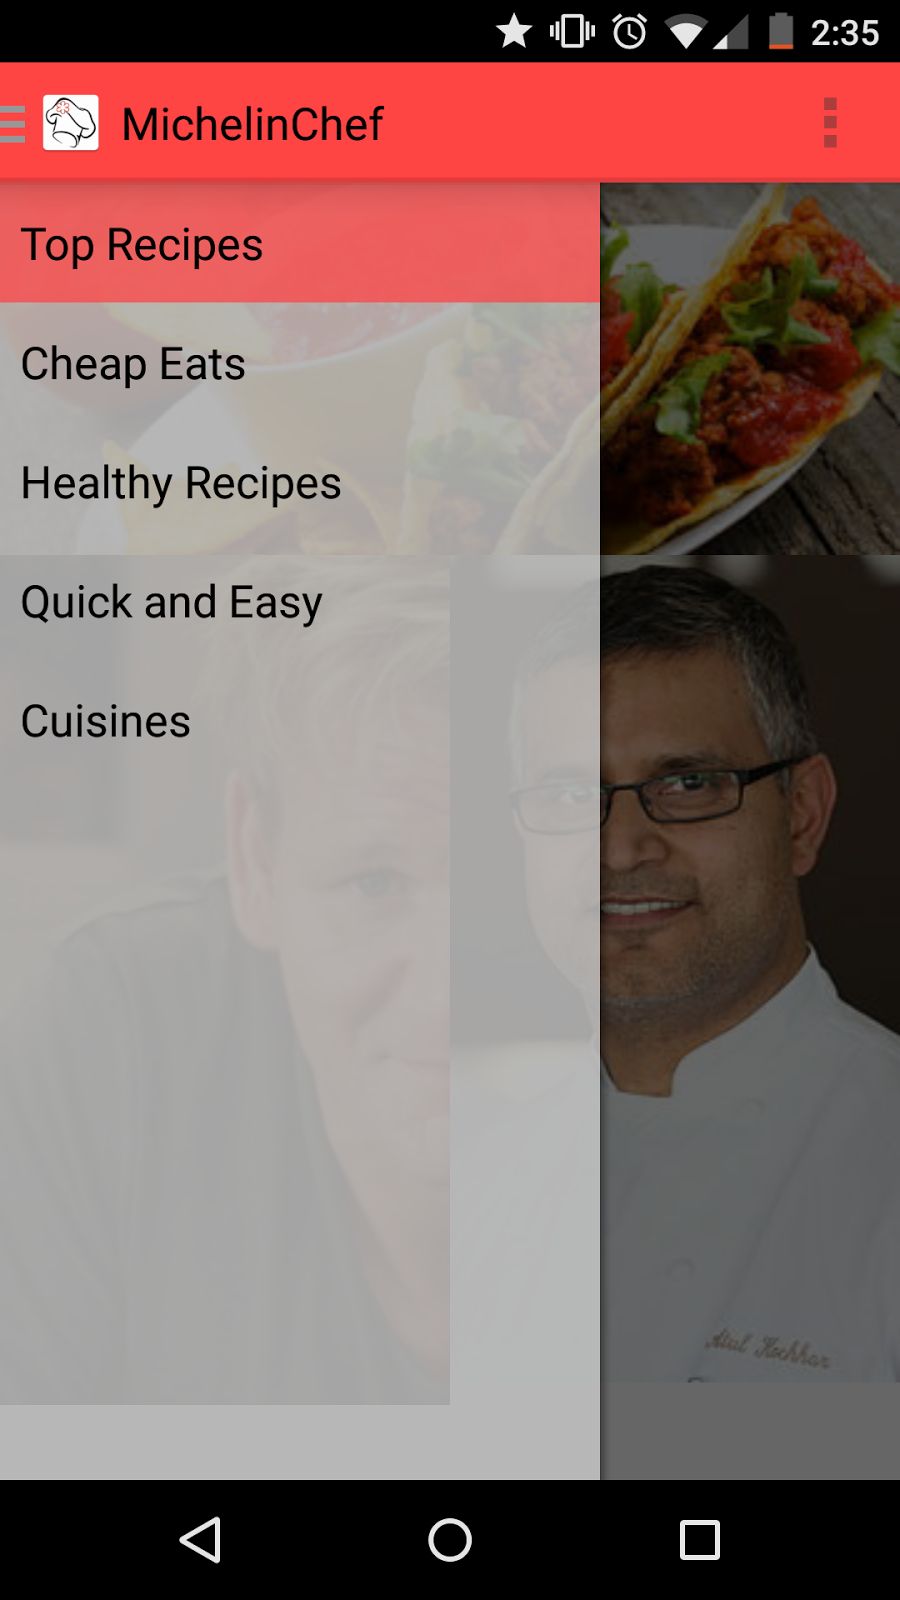
\includegraphics[width=0.3\textwidth, height=0.3\textheight]{images/nav_draw.png}
	\caption{Navigation Drawer to access the different categories of menus\label{fig_1}}
\end{figure}

\begin{figure}[ht!]
	\centering
	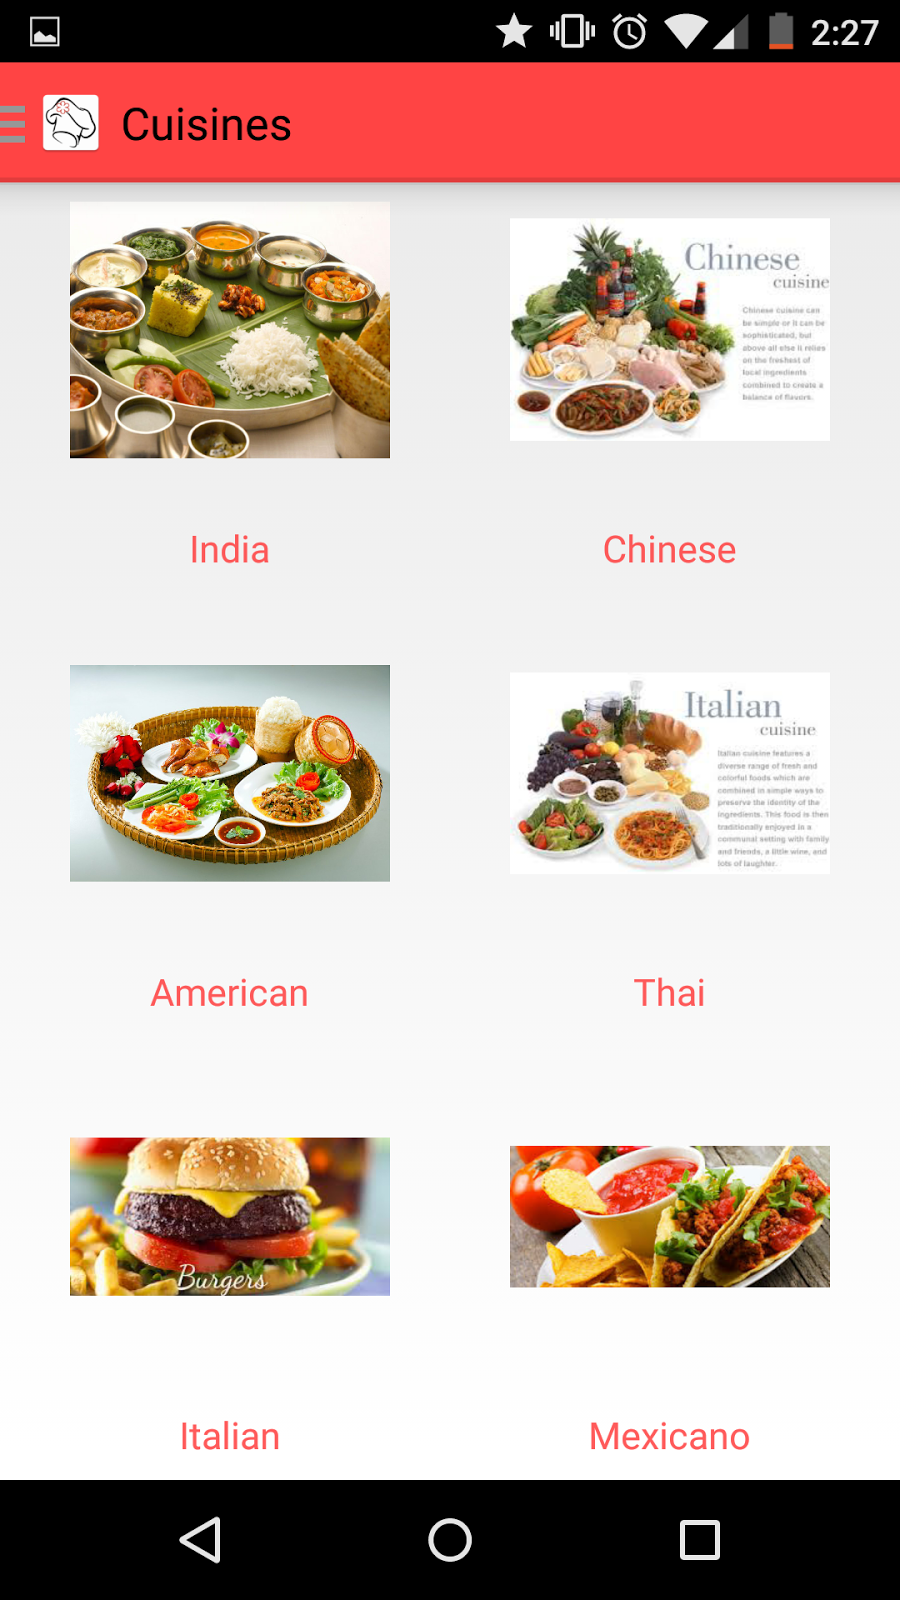
\includegraphics[width=0.3\textwidth, height=0.3\textheight]{images/cuisines.png}
	\caption{Origin based categorization of cuisines\label{fig_2}}
\end{figure}

\begin{figure}[ht!]
	\centering
	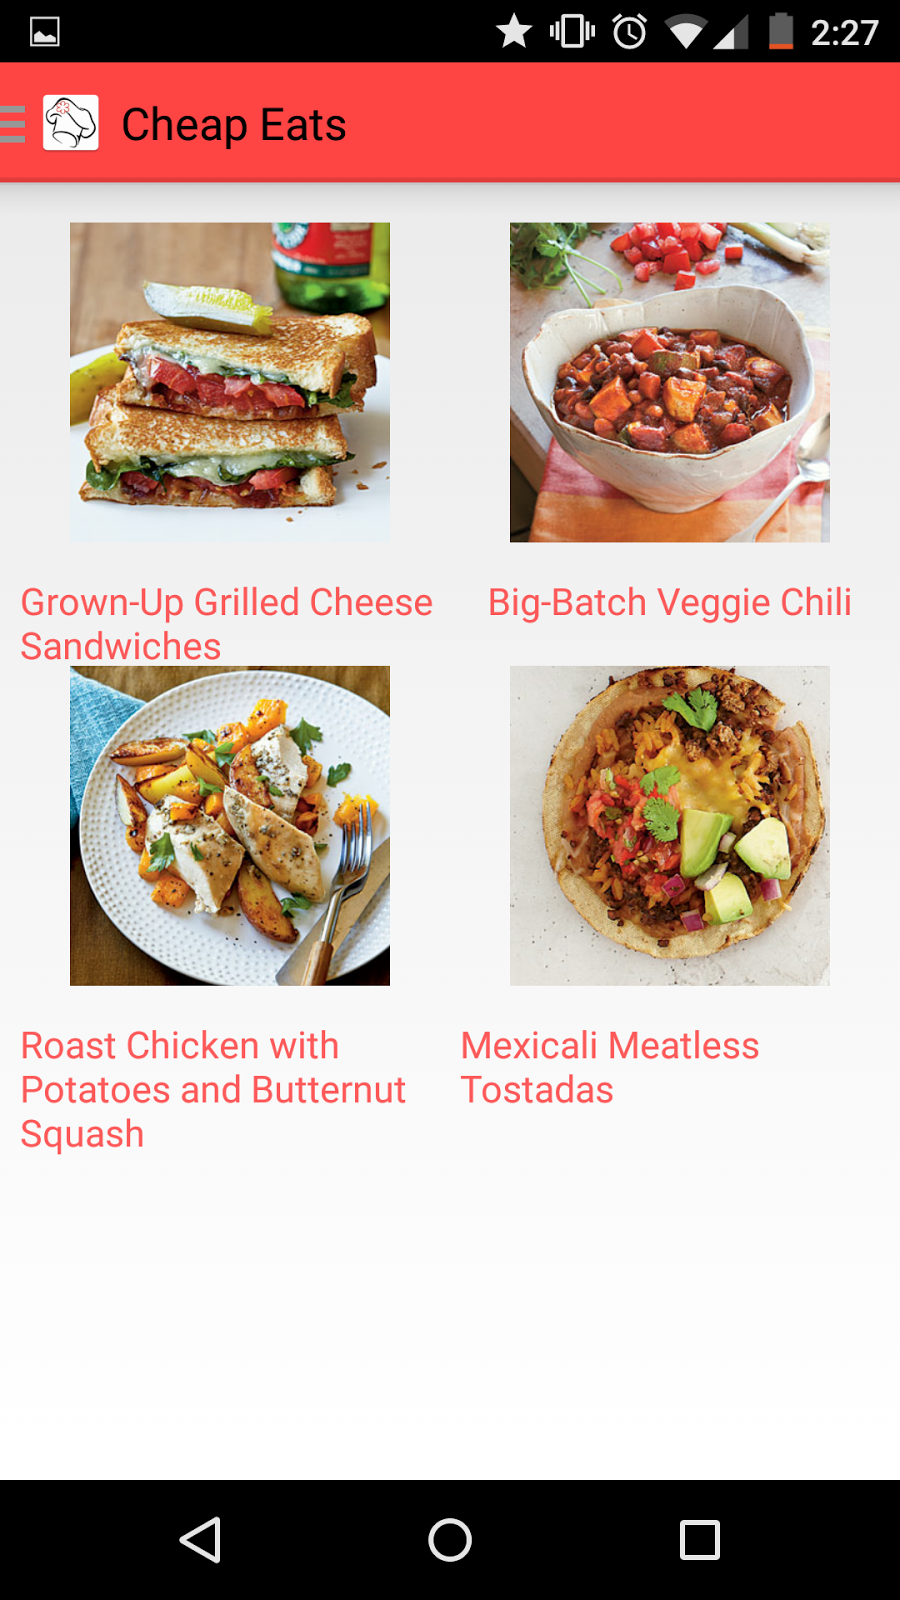
\includegraphics[width=0.3\textwidth, height=0.3\textheight]{images/cheap_eats.png}
	\caption{Different categories of recipes - Cheap Eats\label{fig_3}}
\end{figure}

\begin{figure}[ht!]
	\centering
	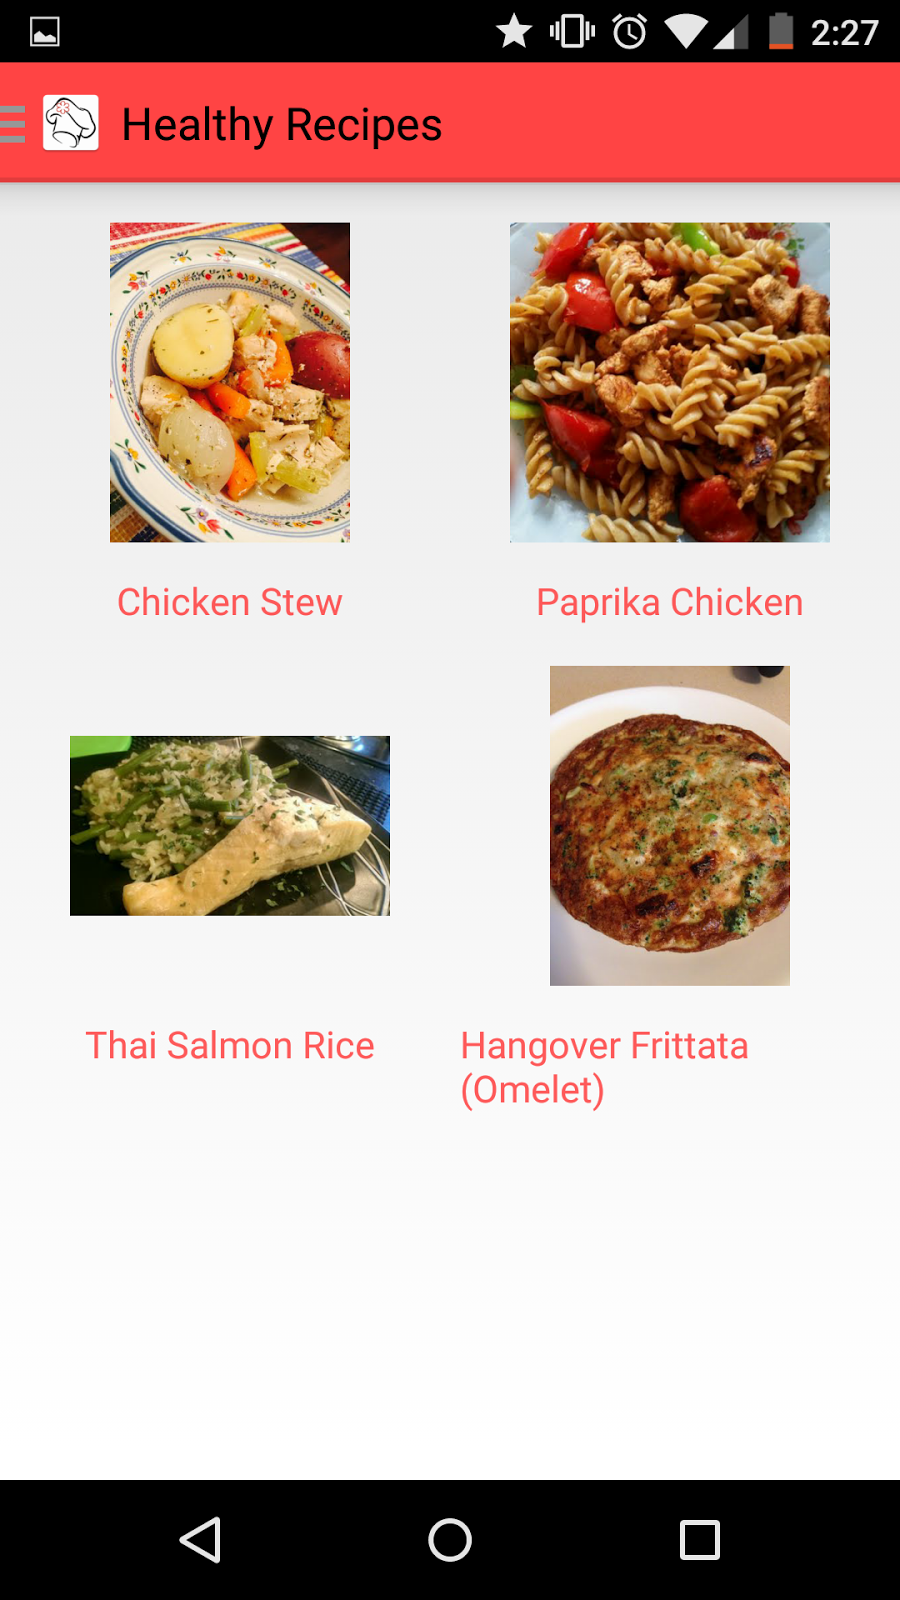
\includegraphics[width=0.3\textwidth, height=0.3\textheight]{images/healthy.png}
	\caption{Different categories of recipes - Healthy\label{fig_4}}
\end{figure}

\begin{figure}[ht!]
	\centering
	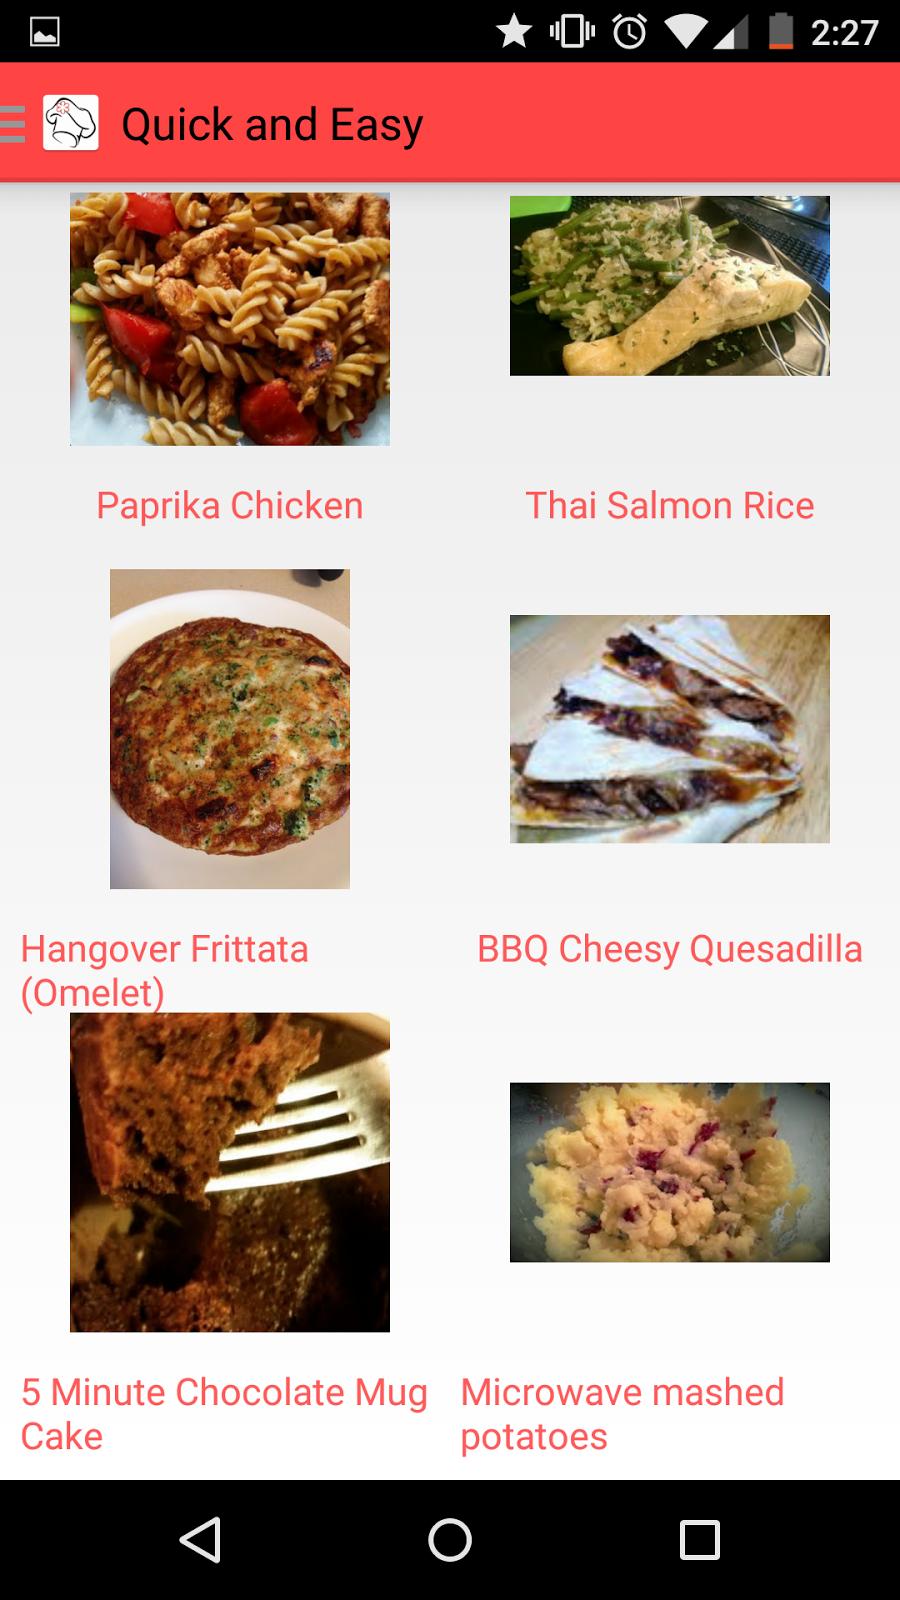
\includegraphics[width=0.3\textwidth, height=0.3\textheight]{images/quick_easy.png}
	\caption{Different categories of recipes - Quick \& Easy\label{fig_5}}
\end{figure}


\begin{figure}[ht!]
	\centering
	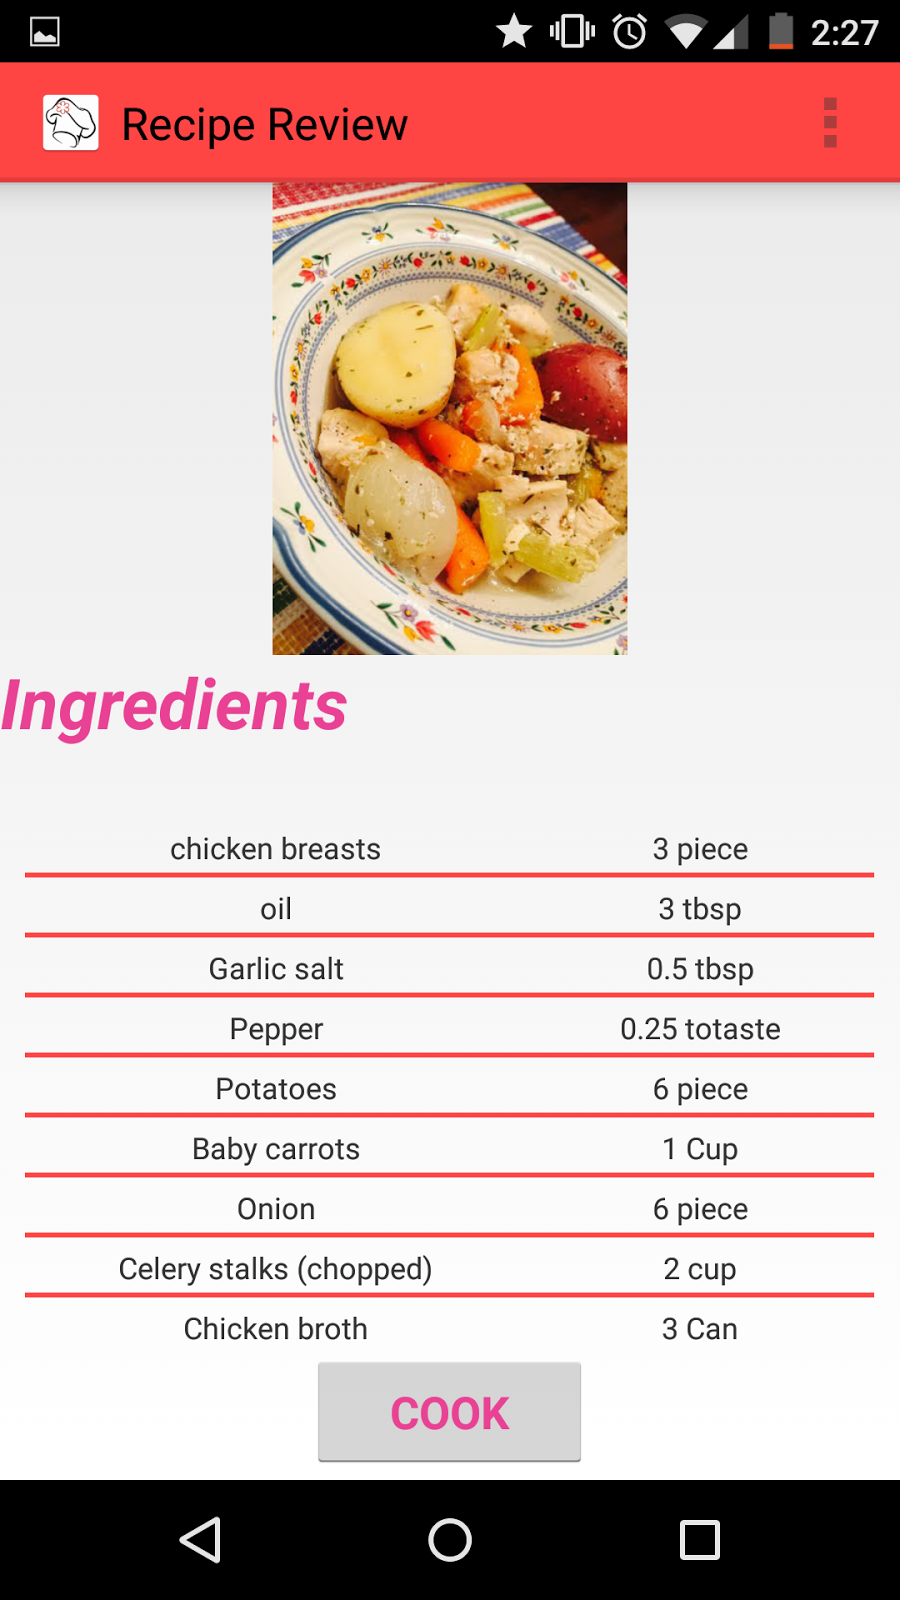
\includegraphics[width=0.3\textwidth, height=0.3\textheight]{images/recipe_review.png}
	\caption{Recipe Review screen that shows the ingredients \label{recipe-review}}
\end{figure}


\begin{figure}[ht!]
	\centering
	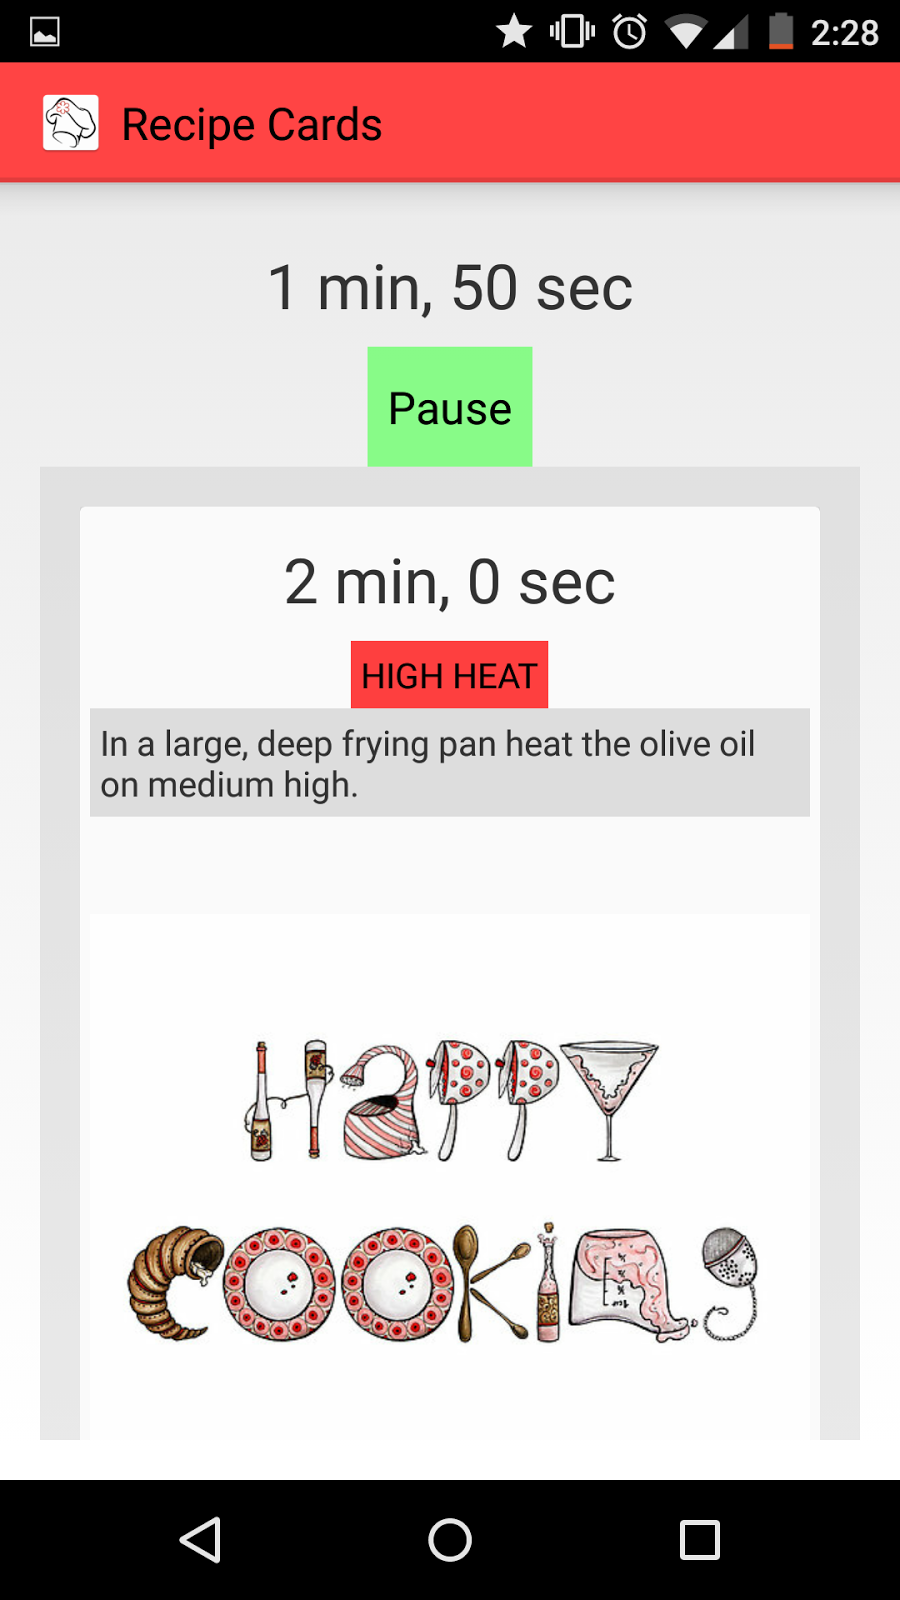
\includegraphics[width=0.3\textwidth, height=0.3\textheight]{images/recipe_cards_1.png}
	\caption{Recipe card that enables easy delivery of cooking instructions \label{recipe-card1}}
\end{figure}

\begin{figure}[ht!]
	\centering
	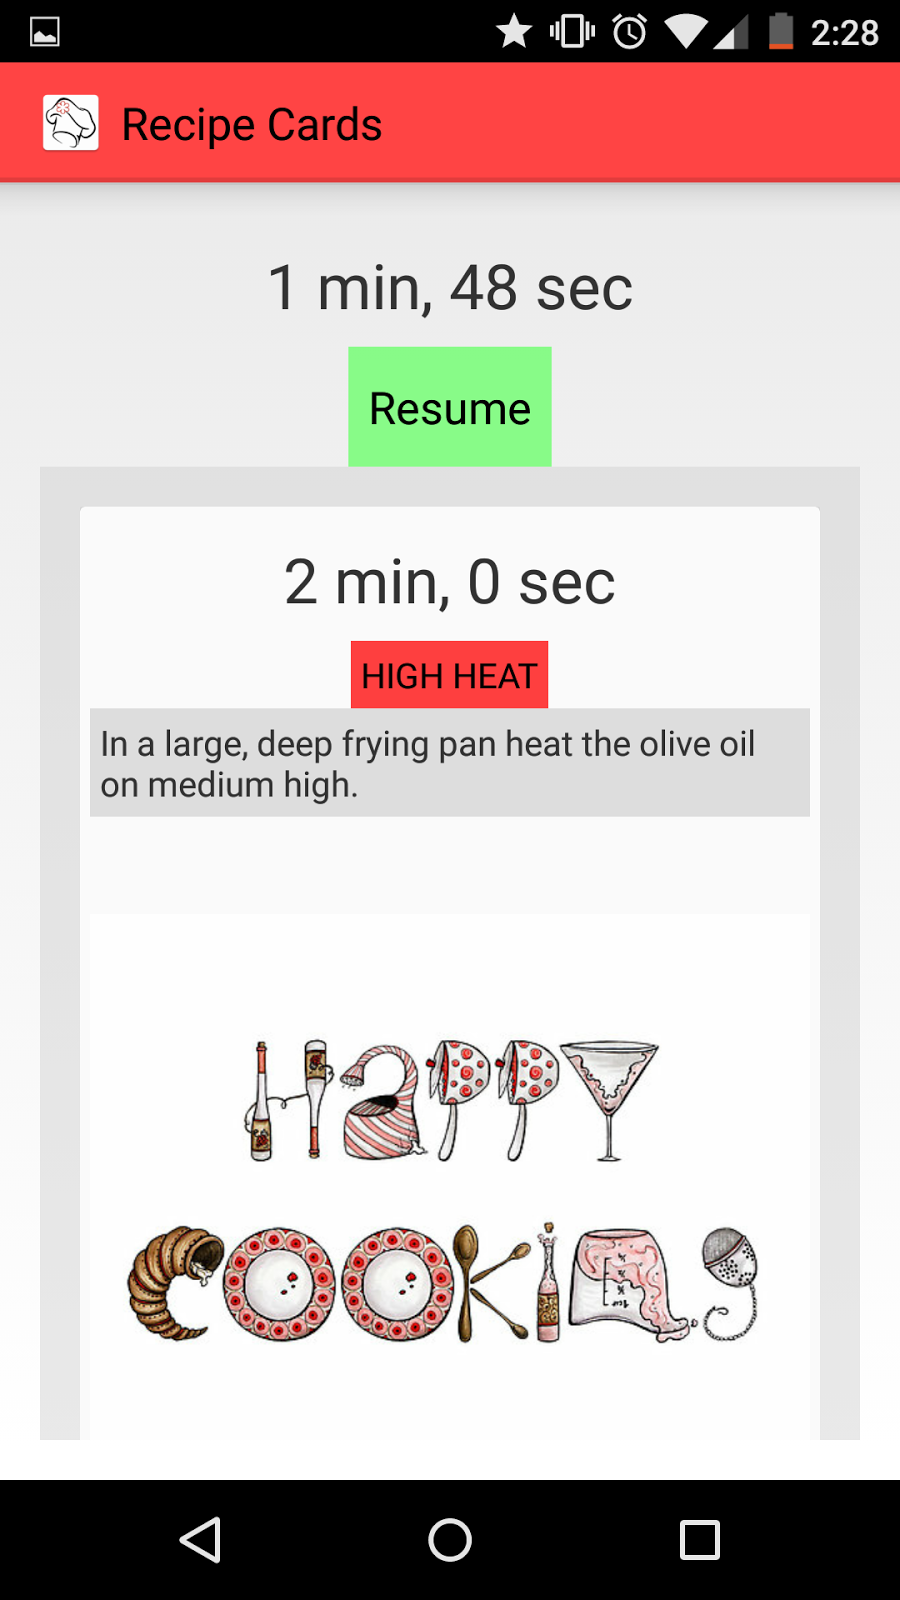
\includegraphics[width=0.3\textwidth, height=0.3\textheight]{images/recipe_cards_2.png}
	\caption{Recipe card that enables easy delivery of cooking instructions \label{recipe-card2}}
\end{figure}

\subsection{Step 2 : Android Implementation}
Following our UI prototyping, we implemented our app using Android Lollipop 5.0 SDK 
\cite{lollipop}. 
In our implementation we used Android framework components such as Fragments \cite
{fragments} and activities \cite{activites}. 
We implemented the following functionality in the app 
\begin{itemize}
\item Different categorization of recipes
\item Recipe review and recipe cards \cite{CardView} for each recipe
\end{itemize}
We implemented two different categorizations 
\begin{enumerate}
\item Quality of food based categorization viz
	\begin{enumerate}
		\item Cheap Eats recipes
        \item Quick and Easy recipes
        \item Healthy food recipes
	\end{enumerate}
\item Origin based categorization viz
	\begin{enumerate}
		\item Indian,
        \item Chinese,
        \item American,
        \item Mexican etc... 
	\end{enumerate}
\end{enumerate}

In order to allow for reuse and to keep the app light on memory consumption, we built all categories over fragments.
A fragment is a reusable part of the application for often re-occurring structures. 
Since the quality of food categories are very similar, we built fragments for each of them and dynamically replace fragments according to user input. 
In order to make navigation as efficient as possible, we built a navigation drawer layout - a structure that launches user action menus by the swipe from the left end of the user interface.
Each of the fragments were tied to this navigation menu.
We also implemented the origin based categorization in a similar fragment.

We also implemented the recipe review screen for each recipe. 
The recipe review screen takes a given recipe as input and displays the end image and the ingredients that are needed. 
The ingredients are taken from the database and are displayed in a user-friendly manner (table).
After reviewing the recipe ingredients, the chef can click on the 'Cook' button. 
Once it is clicked, the digital cards are displayed to the user.
The user can review all the steps required for the recipe and read through the entire layout once if he so desires.
Once the chef is ready to cook, he may click the 'Start' button and the timer starts.
Each step of the recipe has a timer associated with it. When the user clicks the 'Start' button, the first step timer is fired and is counted down. Once it is complete, the step is removed from user view (via scrolling) and the next step is shown and the next step's timer is now fired. 
This is repeated for all steps until the last step. Once all the timers run out, the recipe is completed. In addition, the chef is allowed to pause/resume the flow of cards according to his/her will.

\subsection{Step 3: Database Implementation}

\begin{figure*}[ht!]
	\centering
	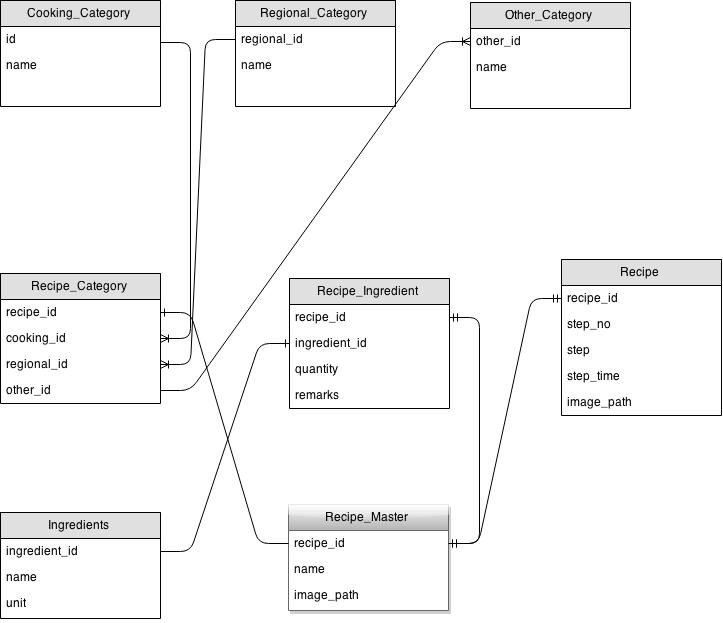
\includegraphics[width=0.8\textwidth, height=0.4\textheight]{images/db.jpg}
	\caption{Database scheme \label{db-schema}}
\end{figure*}

We have used Android SQLite database for this application. SQLite is a very light weight database which comes with Android OS. Basic Database design for the application is as follows (and shown in Figure \ref{db-schema}).

\begin{enumerate}
\item Cooking\_Category : This is a master table for recipe categories based on cooking method. It contains category id and name where id is the primary key.	


\item Regional\_Category :  This is a master table for recipe categories based on regional origin of the recipe. It contains regional category id and name where id is the primary key. 
\item Other\_Category : This is a master table for other recipe categories such as Quick \& Easy, Cheap eats or Healthy Recipes. It contains category id and name where id is the primary key. 
\item Ingredients : This table contains all the ingredients for all of the recipes inside database. This table contains id, name and quantity unit of the ingredient where id is the primary key.
\item Recipe\_Master : Recipe\_Master table is master table where all the recipes, their ids and display image paths are stored. Recipe\_id is the primary key of this table.
\item Recipe\_Category : This table contains information about which recipe belongs to which category. It contains recipe\_id, cooking\_id, regional\_id and other\_id which all are Foreign keys of Recipe\_Master, Cooking\_Category, Regional\_Category and Other\_Category tables respectively.
\item Recipe\_Ingredients : This table contains list of ingredients for each recipe along with quantity and any other remarks. recipe\_id and ingredient\_id are the foreign keys from Recipe\_Master and Ingredients tables respectively.
\item Recipe : This table contains all the steps required to perform cooking with step number, step time and image (if available) for each step. Recipe\_id is the foreign key from Recipe\_Master table.
\end{enumerate}

\subsection{Database Integration with the Application}
Once the database was implemented, we integrated our application with it using Android SQLite APIs. We populated our user interface with data read from Database using Database Helper class. In Database Helper class, we have implemented different helper methods that execute SQL queries using rawQuery API of SQLite and retrieve the appropriate recipe data and pass it on our Android activities. 

Recipe categories implemented as Android Fragments such as Cuisines, Quick and Easy, Cheap Eats, Healthy calls their corresponding Database Helper methods. They return data back to these Categories. Once the recipe category fragments receive data from database helper methods they show the content such as recipe text and recipe image to the user. 

When the user clicks one of the dishes, the recipe category Fragment passes the Recipe ID as part of intent object to the Recipe Preview screen activity. The Recipe preview screen activity after retrieving the Recipe ID from the intent object calls Database Helper method with the Recipe ID to retrieve the appropriate list of ingredients and their quantities and Recipe Image on the Recipe preview screen. 

After the user reviews the recipe review screen and decides to cook that dish, they will click the 'Cook' button. When that happens, the same intent bounded with Recipe ID will be passed to Recipe Digital Card activity. Similar to the Recipe preview screen, Recipe Digital card activity retrieves List of recipe steps, time required for each of the recipe steps, Images required for each of the recipe steps from the Database Helper class by passing on the Recipe ID . Essentially, Database helper uses Recipe ID and executes the SQL query on database to get the corresponding results.

\subsection{Step 4: Hardware System Design}
This is an embedded system made up of a cook-top \cite{cook-top}, \cite{cook-top1}, a microcontroller with a Temperature sensor and a Bluetooth module.

\begin{figure*}[ht!]
	\centering
	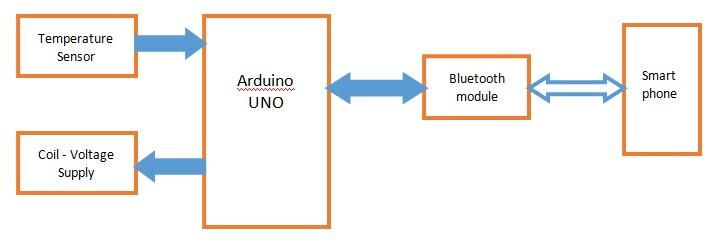
\includegraphics[width=0.8\textwidth, height=0.2\textheight]{images/hw_1.jpg}
	\caption{Top Level design of Smart Cook-Top \label{hw_1}}
\end{figure*}

\begin{figure*}[ht!]
	\centering
	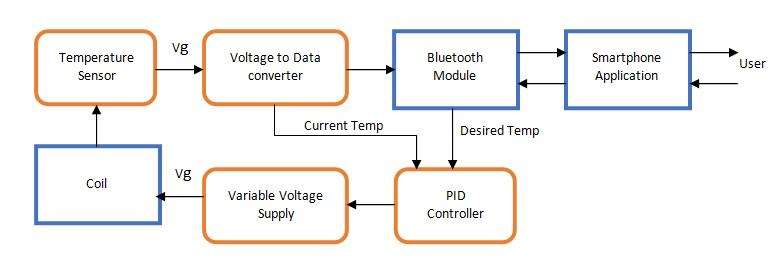
\includegraphics[width=0.8\textwidth, height=0.2\textheight]{images/hw_2.jpg}
	\caption{Data flow model of Smart Cook-Top design \label{hw_2}}
\end{figure*}

The temperature sensor senses the current temperature of the coil and then sends this data in the form of an analog signal(voltage signal ~10mv). The arduino reads the voltage level on the analog input pin available on the board. The voltage level is processed in the arduino and the equivalent temperature information is sent on the serial communication lines to the bluetooth module, this temperature information is then wirelessly transmitted to the paired smartphone. The temperature value can be viewed on MichelinCook.

The desired temperature value of the cook-top is sent from the MichelinCook application to the bluetooth module which is then sent to the arduino module. To set the cook-top to a particular temperature, a PID algorithm is implemented in the arduino, it makes use of the current temperature and the desired temperature values to calculate the required change in the voltage value. The new voltage is supplied to change the temperature in steps till the desired value of temperature is reached. 

The smart cook-top to control temperature and communicate with MichelinCook application was prototyped in simulink. The simulink model was used to simulate the design to check for its working and functionality.

% \begin{figure}[ht!]
% 	\centering
% 	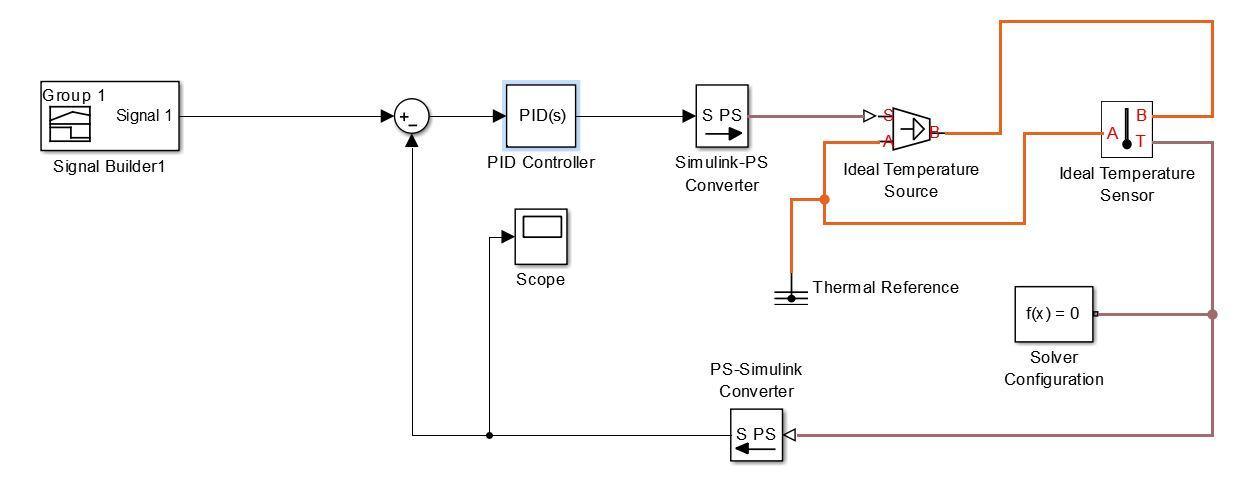
\includegraphics[width=0.4\textwidth, height=0.2\textheight]{images/hw_3.jpg}
% 	\caption{Data flow model of Smart Cook-Top design \label{hw_2}}
% \end{figure}

The signal builder in Fig 13 is configured to present temperature values relative to time. The signal builder has temperature values of 80C from 0s to 300s and 100C from 300s to 1000s. The cook-top coil is modelled as an Ideal temperature source in this phase of the project. The closed system has a PID controller which is a commonly used controller in industries.

The PID values are selected to minimize the rise and have low overshoot as possible. The output of the closed loop system is monitored using the scope. The signal waveform corresponding to input signal from signal builder and output temperature as sensed by the temperature sensor is as shown in figure below.

% \begin{figure*}[ht!]
% 	\centering
% 	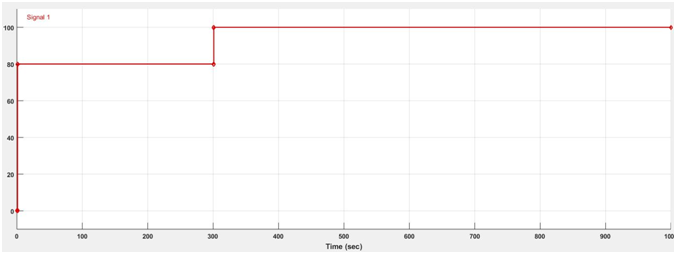
\includegraphics[width=0.8\textwidth, height=0.2\textheight]{images/hw_4.png}
% 	\caption{Output signal given the input signal \label{hw_4}}
% \end{figure*}

% \begin{figure*}[ht!]
% 	\centering
% 	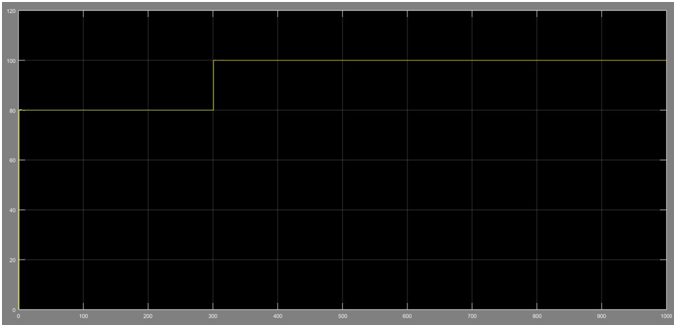
\includegraphics[width=0.8\textwidth, height=0.2\textheight]{images/hw_5.png}
% 	\caption{Mathematical response for real cook-top process\label{hw_5}}
% \end{figure*}

To develop the mathematical response for the real [non ideal] cook-top process is very important. Most processes similar to cook-tops are modelled using First or Second order plus dead time models.

\begin{figure*}[ht!]
	\centering
	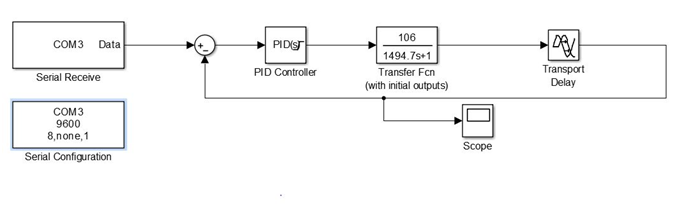
\includegraphics[width=0.8\textwidth, height=0.2\textheight]{images/hw_6.png}
	\caption{Real Cook-Top Design with real cook-top behavior modelled using FODPT \label{hw_6}}
\end{figure*}

\begin{figure*}[ht!]
	\centering
	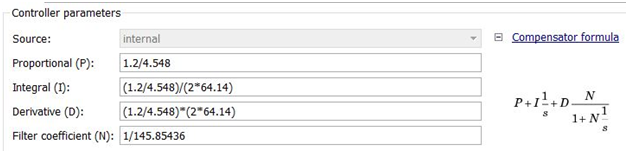
\includegraphics[width=0.8\textwidth, height=0.2\textheight]{images/hw_7.png}
	\caption{PID parameters \label{hw_7}}
\end{figure*}

The response graph for the real cook-top is as shown in the figure below.

% \begin{figure*}[ht!]
% 	\centering
% 	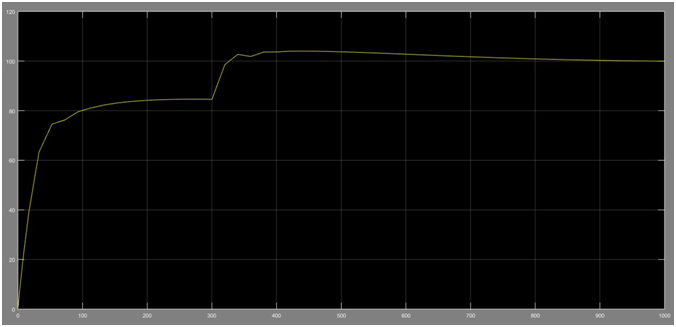
\includegraphics[width=0.8\textwidth, height=0.2\textheight]{images/hw_8.png}
% 	\caption{Temperature response of real(FODPT) cook-top coil \label{hw_8}}
% \end{figure*}





